\documentclass{article}
\usepackage{amsmath}
\usepackage{graphicx}

\title{Rolling a $d_7$ in Finite(ish) Time}
\author{Kevin Berry}

\begin{document}

\maketitle

\par A few years ago, I was hanging out with a couple of friends when they began talking about Dungeons and Dragons.
For those unfamiliar with it, Dungeons and Dragons is a tabletop game which requires many different dice for different situations. 
A typical die set includes a $d_4$, which is a 4-sided tetrahedral die; a $d_6$, a standard 6-sided die; a $d_8$, an octahedrial die; an anomalously non-platonic $d_{10}$, which is the slightly verbosely named pentagonal trapezohedron; a $d_{12}$, a dodecahedron; and a $d_{20}$, which is an icosahedron.
Some people also include the degenerate $d_2$ as part of the die set, even though it is simply a standard 2-sided coin.

\par Since I actually know very little about the game itself, as my friends were talking I began to wonder if there were any interesting conversations to be had about the dice, with which I am much more familiar.
The question that came to mind was essentially this: given only the standard D\&D dice, is it possible to ``roll'' a die with any number of sides? 
In other words, is it possible to generate a number uniformly at random from 1 to $n$, using only a finite set of dice, such as a $d_2$, $d_4$, $d_6$, $d_8$, $d_{10}$, $d_{12}$, or $d_{20}$?
I briefly brought up this question, and we discussed it for a moment.
Alas, I found it more interesting than they did, so here we are.

\par The first die missing from a standard set would be the trivial 1-sided die, which always rolls a 1.
One can pretend to roll such a die by shouting the number ``1'', which is satisfactory for our purposes.\footnote{One could also consider rolling a zero sided die, which one rolls by not considering it.}

\par What about a 3-sided die?
This is a much more interesting case to solve.
It turns out, there are many solutions to rolling a $d_3$.
One way to do this is to roll a $d_6$ and divide the rolled value by 2, rounding up.
This rule means that a roll of 1 or 2 is counted as a 1, a roll of 3 or 4 is counted as a 2, and a roll of 5 or 6 is counted as a 3.
This nicely produces a uniform distribution from 1 to 3, since 1 and 2 are just as common as 3 and 4 or 5 and 6 on a fair $d_6$.
In fact, any function which maps 3 disjoint pairs of faces of a $d_6$ onto the numbers 1 to 3 will work for simulating a roll of a $d_3$ from a roll of a $d_6$.

\par Similarly, one could roll a $d_3$ by mapping 3 disjoint sets of 4 faces from a $d_{12}$ onto the numbers 1 to 3.
What's more, a $d_4$ can be rolled by remapping the faces of a $d_8$, a $d_5$ can be rolled by remapping the faces of a $d_{10}$, and a $d_{10}$ could be rolled by remapping the faces of a $d_{20}$. 
In general, given a die $d_{f_1}$ with $f_1$ faces, it is possibly to roll any other die with a number of faces $f_2$ such that $f_2$ evenly divides $f_1$.
One sufficient mapping in this case is $R_{f_1 \to f_2}(r) = \lceil r / (f_1 / f_2) \rceil = \lceil (r / f_1) \cdot f_2 \rceil$, which takes a roll $r$ from a group of size $f_1$ and maps it uniformly to a group of size $f_2$, producing the desired distribution.
For the sake of concreteness, this mapping for rolling a 5 sided die with a 10 sided one is $R_{10 \to 5} = \lceil r / (10 / 5) \rceil = \lceil r / 2 \rceil = \lceil (r / 10) \cdot 5 \rceil$, which I've written in 3 ways to hopefully reveal my intuitions for the correctness of the mapping.

\par While this trick is neat (and will later come in handy), it only allows us to roll two more dice at the moment.
This brings us to the next challenge: rolling a die with 7 sides. 

\par I've asked this question to several friends and family members, and the first approach that tends to be given is to do something like rolling 7 six-sided dice and dividing by 6, rounding down when necessary.\footnote{This was also my first approach.}
At first this may seem to work, but fails upon closer inspection.
The lowest value it outputs is $\lfloor 7 \cdot 1 / 6 \rfloor = 1$, and the highest value it outputs is $\lfloor 7 \cdot 6 / 6 \rfloor = 7$, so the function outputs values in the correct range.
However, the distribution of these values is uneven.
For instance, there are many ways of rolling a 1, such as by rolling six 1s and one 2 or five 1s and two 2s, but the only way to roll a 7 is by rolling 7 sixes.
Clearly, then, this does not generate a random number uniformly from 1 to 7.

\par What about something like rolling a $d_3$ (using a $d_6$, via our earlier method) and a $d_4$ and adding them together?
Well, this nicely has a maximum value of 7, but falls apart when you realize that the minimum value is 2, which is no good.
However, rolling these two dice in this way has another, more insightful flaw.
When rolling a $d_3$ and a $d_4$, there are $3 \cdot 4 = 12$ possible outcomes: $$(1, 1), (1, 2), (1, 3), (1, 4), (2, 1), (2, 2), (2, 3), (2, 4), (3, 1), (3, 2), (3, 3), (3, 4).$$
However, the distribution we aim to recreate has 7 options which must be equally likely.
By the pigeonhole principle, it is clear that an onto mapping from 12 inputs to 7 outputs cannot be done in such a way that all 7 outputs are equally likely; there will be at least two outputs which only have one input mapped to them, and there will be at least one output which has more than one input mapped to it, making that output more likely than at least one other.
Similarly, it is never possible to produce a perfect mapping from a $d_{f_1}$ to a $d_{f_2}$ when $f_2$ is not divisible by $f_1$.
Clearly, then, any perfect rolling scheme which we come up with must have a number of outcomes which is divisible by the number of faces on the die that we want to roll, as was the case with our trick for rolling a $d_3$.

\par While the $d_3$, $d_4$ combination failed to produce a way of rolling a $d_7$, there is another insight to be gleaned from this attempt.
Namely, that we can roll a die whose face count is any product of the face counts of the dice we have. 
This follows from the fact that we can simply enumerate $f$ outcomes of equal probability in order to roll a die with $f$ faces, and rolling a set of dice yields a number of equally likely outcomes which is the product of their number of faces.
With this technique, and the fundamental theorem of arithmetic, we now realize that we only need to be concerned with being able to roll dice with a prime number of faces, since we can generate all other numbers from these.

\par Which brings us back to rolling a 7.
Despite the niceness and utility of our previous observations, we will need some new technique to solve this problem. 
Because of my familiarity with $d_6$s, I first thought of a solution which used only them.
Namely, we can roll two $d_6$s and treat one as the ones digit of a base 6 number (offset by 1) and the other as the sixes digit of a base six number (also offset by 1), and we can just re-roll if we get a value greater than or equal to 7.
This, perhaps, seems a bit obtuse, but is illustrated well by example.
Lets say that we rolled a 4 and then a 3. 
We treat the first number as the number of sixes that we have, plus one, giving us $(4 - 1) \cdot 6 = 18$ to start.
Then, we treat the second number as the number of ones we have, plus one, bringing our total up to $18 + (3 - 1) \cdot 1 = 20$.
If we had rolled two sixes, we would get $(6 - 1) \cdot 6 + (6 - 1) \cdot 1 = 35$, and if we had rolled two ones, we would have gotten $(1 - 1) \cdot 6 + (1 - 1) \cdot 1 = 0$. 
Because each roll in this fashion gives us a unique number on this interval, this scheme gives us each number from 0 to 35 exactly once.
Thus, each of the numbers from 0 to 6 is equally likely, and we can generate a number from 1 to 7 uniformly at random by remapping the numbers 0 through 6 and ignoring and re-rolling for numbers greater than 6.
It may seem like cheating to re-roll, but the reason that it works is that at any time that the dice are rolled, there is always an equal chance of getting the 7 outcomes we care about, and we ignore all other outcomes.
It is also easy to see how we can use this technique to roll \textbf{any die we want.}
For any desired die $d_{f_2}$ and a given die $d_{f_1}$, we can roll $d_{f_1}$ a total of $\lceil \log_{f_1}{f_2} \rceil$ times and treat each roll as a digit of a base $f_1$ number, re-rolling if we roll a number greater than or equal to $f_2$.

\par At this point, an astute reader may notice some peculiarities with this scheme. 
First, wouldn't it have been simpler to roll a $d_7$ by rolling a $d_8$ and re-rolling only when an 8 is rolled? 
Yes, it would've been, but I didn't think of that until later.
Second, can't this rolling scheme go on infinitely if we always roll a value which is too high?
Yes!
However, thankfully, this almost surely never happens, which is to say that the probability that this happens approaches 0 in the limiting case of the number of rolls approaching infinity.
For any scheme where each roll is independent of the previous and we have $T$ possible outcomes and we accept $t$ of them and re-roll on the other $T - t$, the probability of rolling $n$ rejected values in a row is $\left(\frac{T - t}{T}\right)^n$, which goes to 0 as $n$ approaches infinity, since $T - t$ is clearly positive and less than $T$, making $0 < \frac{T-t}{T} < 1$. 

\par We can also compute the expected number of throws (how many times we have to roll a set of dice) based on the probability of needing to throw again.
Using the same $t$ and $T$ as before, we have to consider the number of throws if we succeed on the first throw and the number of throws if we fail on the first throw.
In either case, we have to throw at least once. 
In the case that we succeed, we're done, so our total is one throw.
If we fail, we're back at the beginning, so we have one throw, and we expect to throw the same number of times as if we hadn't thrown at all.
Mathematically, this leads to the equation $$E(\theta) = \frac{t}{T} \cdot (1 + E(\theta | \text{success})) + \left(1 -\frac{t}{T} \right) \cdot (1 + E(\theta | \text{failure}))$$
Since $E(\theta | \text{success}) = 0$ and $E(\theta | \text{failure}) = E(\theta)$, this equation simplifies to be: $$E(\theta) = \frac{t}{T} + \left(1 - \frac{t}{T} \right) \cdot (1 + E(\theta))$$
We can actually solve this algebraically to find that $E(\theta) = T/t$. 
In the case of rolling a 7 sided die with a 6 sided die with 36 outcomes, as described above, the expected number of throws is thus 36/7, which is about 5.14 throws, while rolling a $d_7$ with a $d_8$ results in only $8/7 + 1 \approx 1.14$ throws.
Thus, rolling an 8 sided die is clearly better in expectation.

\par This leads us to a scarier question: can we do better?
Clearly, if we were to get $T$ closer to $t$, then the fraction $T/t$ would decrease, and our expected number of throws would decrease accordingly. 
We can do this by being slightly clever.
While a $d_8$ seems to do better than two $d_6$s at first, we can reuse the trick we used for rolling a $d_3$ with a $d_6$ to make rolling two $d_6$s the better option.
If we take each of our 36 outcomes and map 5 of them to the value 1, 5 of them to the value 2, etc., then we end up with 7 equally likely groups of 5 outcomes each, with only one outcome left over where we need to re-throw.
This means that we only need to throw $36/35 \approx 1.03$ times on average! 
We could even resort to using different pairs of dice, such as a $d_6$ and a $d_{20}$.
This gives us 120 outcomes, which we can break up into 7 groups of 17 with one left over, giving us an expectation of only $120/119 \approx 1.01$ throws.

\par The next follow-up question to this is whether or not we can achieve arbitrarily few throws for 7, or any number in general. 
It's actually fairly easy to show that this is the case.
For example, take a die with any number of faces $f_2$ that we want to roll, and $n$ dice with $f_1$ faces each.
We can throw all of the $n$ dice, giving us $f_1^n$ outcomes.
Assuming $f_1^n$ is greater than $f_2$, we can then break these outcomes into $f_2$ groups with $r$ outcomes left over, where we would need to re-throw.
This gives us an expected number of throws $$E_n(\theta) = \frac{T}{t} = \frac{f_1^n}{f_1^n - r} = \frac{1}{1 - r/f_1^n},$$ which approaches 1 as $n$ approaches infinity since $r/f_1^n$ approaches 0 as $n$ approaches infinity.

\par Another question one might ask is how few throws we can achieve using only finitely many dice.
In general, we'll try to roll a $d_{f_2}$ with a given a set of dice $D$. 
The total number of outcomes $T$ for this set of dice will simply be the product of the number of faces of the dice in the set, $\Pi_D=\prod_{d_{f_1}\in{D}}f_1$.
If we use the same grouping trick as earlier, then the number of outcomes $t$ where we don't need to re-roll is the greatest integer multiple of $f_2$ which is less than $\Pi_D$.
More precisely, we will not need to re-roll for $f_2\lfloor \Pi_D/f_2\rfloor$ of the possible $\Pi_D$ outcomes. 
Thus, we will have an expected number of throws: $$E_D(\theta) = \frac{T}{t} = \frac{\Pi_D}{f_2\lfloor \Pi_D/f_2\rfloor}$$
Perhaps surprisingly, it is always better to roll the entire set of dice $D$ than it would be to roll any subset of $D$. 
To prove this, it is sufficient to show that adding another die will never increase the number of expected rolls, since this will then allow us to include dice until we have included the entire set $D$.
If we add any die $d_{f_3}$ to the set $D$, giving us the set $D\cup \{d_{f_3}\}$, then our expectation becomes: $$E_{D\cup\{d_{f_3}\}}(\theta) = \frac{f_3 \cdot \Pi_D}{f_2\lfloor f_3 \cdot \Pi_D/f_2\rfloor}$$
We now want to show that this value is never more than the expectation without $d_{f_3}$. 
Comparing the two and simplifying, we find:
\begin{align}
\frac{f_3 \cdot \Pi_D}{f_2\lfloor f_3 \cdot \Pi_D/f_2\rfloor} & \leq\frac{\Pi_D}{f_2\lfloor \Pi_D/f_2\rfloor}\\
\frac{f_3}{\lfloor f_3 \cdot \Pi_D/f_2\rfloor} &\leq \frac{1}{\lfloor \Pi_D/f_2\rfloor}\\
f_3 \lfloor \Pi_D / f_2 \rfloor &\leq \lfloor f_3 \Pi_D / f_2 \rfloor
\end{align}
If we let $v = \Pi_D / f_2$ and $u = f_3$, then line 3 is equivalent to $u \lfloor v \rfloor \leq \lfloor uv \rfloor$.
In the case that $u$ and $v$ are both integers, the equality holds.
Because $u = f_3$ is the number of faces on the added die, and thus always an integer, the only other case to consider is when $v$ is not an integer.
In this case, $u \lfloor v \rfloor$ will be exactly $u$ times the integer portion of $v$, while $\lfloor uv \rfloor$ will be \textbf{at least} $u$ times the integer portion of $v$, since the rounding down is done after computing $uv$.
Thus, the inequality in line 3 is true for all $D$, $f_2$ and $f_3$, completing the argument that adding another die never increases the expected number of rolls.

\par These answers are not fully satisfying, however.
While we can get the number of total throws arbitrarily close to 1, the total number of dice rolled simultaneously approaches infinity, which is, in some respects, impractical.
A more satisfying answer would minimize the total number of dice ever rolled, rather than the number of throws.\footnote{Another more satisfying answer would be to try to simultaneously minimize the number of throws and the number of dice rolled, but the optimal answer in this case is possibly subject to a preference of which value is more important to minimize.}
The expected number of dice rolled is simply the expected number of throws, multiplied by the number of dice rolled in each throw.
For a general set of dice $D$, as defined above, the expected number of rolls is simply $E_D(r)=|D|E_D(\theta)$.
However, unlike minimizing the number of throws, it is easy to construct examples where there are subsets $S$ of $D$ that result in fewer rolls in expectation than the full set $D$.
Unfortunately, it seems to be a computationally difficult task to find the subset $S$ which actually minimizes this expectation.
Because for each die in $D$ we have a binary choice of whether or not to include it in a subset $S$, there will be $2^{|D|}$ subsets of $D$ which we may need to consider.\footnote{This follows from the fact that the number of binary strings of length $n$ is $2^n$ and we can represent each set as a binary string of length $n=|D|$, with a 1 if a die is included and a 0 if it is excluded.}
Na\"ively examining each of these subsets individually takes exponential time and becomes intractible for even small sets of dice, e.g., 30 dice, for which there are 1,073,741,824 possible subsets.
A slightly less na\"ive algorithm for computing the optimal subset might be to consider only the subsets whose product is at least $f_2$, though this could still comprise every or nearly every subset of $D$, such as in the event that each element of $D$ has a face value of at least $f_2$.
Because of the floor function in the expectation, there is no optimal substructure to the problem which would allow us to eliminate groups of candidate subsets at a time, as would normally done with dynamic programming.
Thus, it seems that there is no easy way to compute the optimal number of throws for an arbitrary subset of given dice efficiently.

\par Despite this, an interesting and computationally efficient case to analyze is when we have an unlimited set of the same die.
For a set of $n$ dice each with a face value of $f_1$ there are $T = f_1^n$ outcomes and $t = f_1^n \left\lfloor \frac{f_2}{f_1^n} \right\rfloor$ outcomes where we need to re-roll.
This gives us the following expression to minimize: $$E_n(r) = nE_n(\theta)= \frac{nT}{t} = \frac{nf_1^n}{f_2 \left \lfloor \frac{f_1^n}{f_2} \right \rfloor}$$
Yuck! 
That floor function and those exponents don't look very friendly, and it turns out that they complicate things significantly.
Some of the problems with this minimization become more apparent when we actually graph this as a function of $n$ for particular values of $f_1$ and $f_2$, as shown in figure \ref{fig:num-rolls}.
\begin{figure}
    \centering
    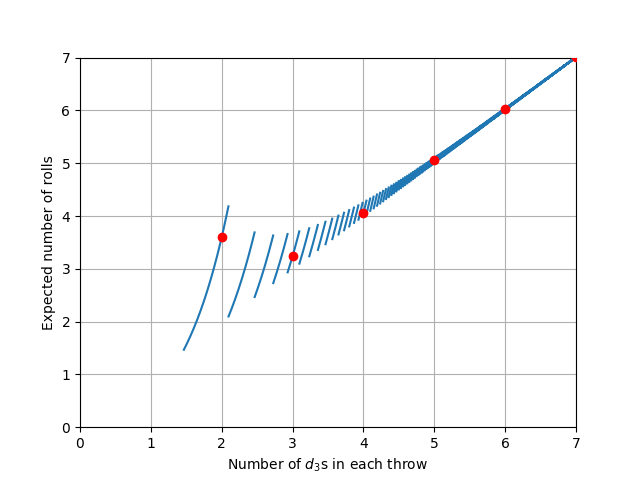
\includegraphics[scale=0.5]{num-rolls.png}
    \caption{Expected number of dice rolled with $f_1=3$ and $f_2=5$. Integer values are shown in red.}
    \label{fig:num-rolls}
\end{figure}
The most obvious problem with the function is that it is not continuous; the floor function in the denominator makes the function discontinuous for infinitely many values of $n$.
Despite the fact that the graph is piecewise monotone increasing, these discontinuities introduced by the floor function mean that we cannot use information about the slope of the graph in any obvious way to find its minimum values.
We also care in particular about integer values of the function, which are evidently not the minima one would obtain from the function when considering non-integer values as well.
Quite a predicament!
\par In order to make some progress on this, it will help to note the bounds of the function.
In order to find the upper bound of $E_n(r)$, we need to minimize its denominator.
Because the denominator corresponds to the number of outcomes where we don't need to re-roll, we can write it as $f_1^n - r$, where $r$ is the remainder of $f_1^n / f_2$, corresponding to the number of outcomes where we do need to re-roll.
Since the remainder is bounded above by $f_2$, we find that $E_n(r)$ is bounded above by $\frac{nf_1^n}{f_1^n-f_2}$, i.e., $E_n(r) \le \frac{nf_1^n}{f_1^n-f_2}$.
Next, to determine the lower bound, we divide the numerator and denominator of our equation by $f_1^n$ to get: $$E_n(r) = \frac{n}{\frac{f_2}{f_1^n} \left \lfloor \frac{f_1^n}{f_2} \right \rfloor}$$
Since the numerator here is $n$ and the denominator is always between 0 and 1, we find that the function is bounded below by $n$, i.e., $E_n(r) \ge n$.
The graph of this expectation is shown with its bounds in figure \ref{fig:num-rolls-with-bounds}.\footnote{It is worth noting that the upper bound has an asymptote where $f_1^n=f_2$; to the left of this asymptote, values of the function are negative, so we ignore them.}
\begin{figure}
    \centering
    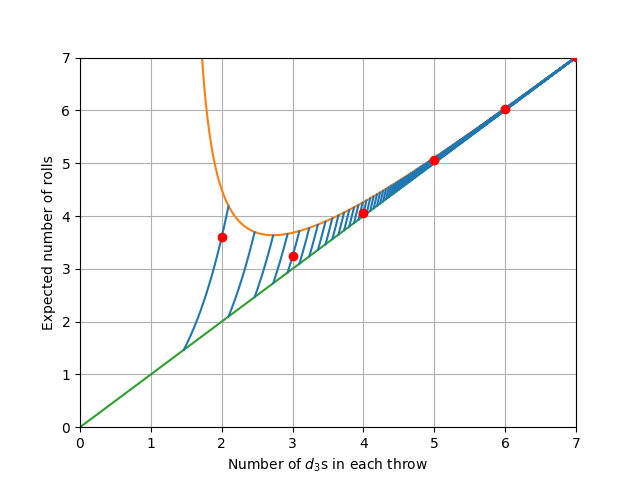
\includegraphics[scale=0.5]{num-rolls-with-bounds.png}
    \caption{Expected number of dice rolled with $f_1=3$ and $f_2=5$. Integer values are shown in red. Upper bound is shown in orange, lower bound in green.}
    \label{fig:num-rolls-with-bounds}
\end{figure}
\par It is easy to see that the both the lower and upper bounds of the number of dice rolled both approach $n$ as $n$ grows large.
In other words, as the number of dice in each throw grows large, we expect to eventually have one throw consisting of all of the dice.
Since the bounds are both increasing and become arbitrarily close to each other, it follows that there is some minimum value $m$ such that $E_n(r) > E_m(r)$ for all $n > m$.
If we could find this $m$, we would only need to check values less than it to determine which one minimizes the expected number of rolls.
Thus, it seems useful to find when $E_n(r)$ always increases when we add another die, i.e., $E_{n+1}(r) > E_n(r)$ for all positive integers $n > m$.
For this, we can subtract the upper bound for $E_n(r)$ from the lower bound for $E_{n+1}(r)$, since this is the smallest the difference between consecutive terms could possibly be.
Through some tedious algebra, we find:
\begin{align}
    E_{n+1}(r) - E_n(r) &> 0 \\
    (n + 1) - \left( \frac{nf_1^n}{f_1^n - f_2} \right) &> 0 \\
    \frac{nf_1^n + f_1^n-nf_2-f_2}{f_1^n-f_2} - \frac{nf_1^n}{f_1^n - f_2} &> 0 \\
    \frac{(f_1^n-f_2) - nf_2}{f_1^n-f_2} &> 0 \\
    1 - \frac{nf_2}{f_1^n-f_2} &> 0 \\
    f_1^n &>nf_2 + f_2
\end{align}
While the last line here might not look too complicated, it should be apparent that we cannot easily eliminate the exponential term from this equation.
Those familiar with exponential equations may recognize that we will need to resort to using the Lambert W function in order to solve for $n$.
To those unfamiliar with exponential equations, this is the function $W$ such that $W(ve^v)=v$ for any expression $v$. 
While the W function cannot be expressed in terms of elementary functions, it is practical to evaluate because its values can be computed easily via Newton's method.
It will be useful for our purposes if we can get the exponential portion of our equation into a ``canonical'' form, i.e., the form $C(n)e^{C(n)}$, where $C$ is some non-exponential function of $n$, since we can then apply the relation $W(C(n)e^{C(n)})=C(n)$ to eliminate the exponentials from our equation.
This results in the following manipulations, all of which are simply convincing the coefficient of the exponential term to look more and more like the exponent of the exponential term:
\begin{align}
    1 &< (nf_2+f_2)f_1^{-n} \\
    -1 &> (-nf_2-f_2)f_1^{-n} \\
    -1 &> (-nf_2-f_2)e^{-n\log{f_1}} & \text{by } a^x=e^{x\log{a}}\\
    -\log{f_1} &> (-nf_2\log{f_1}-f_2\log{f_1})e^{-n\log{f_1}}\\
    -\frac{\log{f_1}}{f_2} &> (-n\log{f_1}-\log{f_1})e^{-n\log{f_1}}\\
    -\frac{\log{f_1}}{f_2}e^{-\log{f_1}} &> (-n\log{f_1}-\log{f_1})e^{-n\log{f_1}-\log{f_1}}\\
    -\frac{\log{f_1}}{f_1f_2} &> (-n\log{f_1}-\log{f_1})e^{-n\log{f_1}-\log{f_1}}
\end{align}
Now, the right hand side is in the canonical form with $C(n) = -n\log{f_1}-\log{f_1}$, so we can apply the $W$ function to both sides and simplify:
\begin{align}
    W\left(-\frac{\log{f_1}}{f_1f_2}\right) &> -n\log{f_1}-\log{f_1}\\
    \frac{W\left(-\frac{\log{f_1}}{f_1f_2}\right) + \log{f_1}}{\log{f_1}} &> -n\\
    \frac{W\left(-\frac{\log{f_1}}{f_1f_2}\right)}{\log{f_1}} + 1 &> -n\\
    -\frac{W\left(-\frac{\log{f_1}}{f_1f_2}\right)}{\log{f_1}} - 1 &< n
\end{align}
meaning that for all $n$ greater than the value of the left hand expression, $E_{n+1}(r) > E_n(r)$.
With this (fairly complicated) expression,\footnote{This expression is even more complicated than I'm letting on. Since the W function is multi-valued, we need to be careful to take the value which makes the number of expected rolls positive.} we now have a limited set of candidates to check to find the integer number of dice which globally minimizes the expected number of dice rolled.
We only need to check the few values between $\lceil \log_{f_1}{f_2} \rceil$ and this value, since all possible larger numbers will require more rolls in expectation.
Because $xe^x$ grows faster than $e^x$, the $W$ function grows slower than the logarithm function, meaning that we only have to consider $O(\log{f_1} + \log{f_2})$ possible minimum values, significantly fewer than the exponential number we need to consider with arbitrary sets of dice.

\par There is one last trick\footnote{As far as I know.} that we can use to reduce the expected number of rolls in general.\footnote{Credit for this idea goes to Kenneth Adams.}
When we have a set of dice $D$ such that the product of their faces $\Pi_D = f_2 + r$, we can ``reuse'' rejected rolls.
Specifically, there will be $r$ possible rolls which are rejected, which we can enumerate.
Since each of these rolls is equally likely, we can treat the enumerated value of the rejected roll as an extra roll of a $r$ sided die on our next roll.
For instance, if we were rolling a $d_{13}$ with a $d_{20}$ and we rolled a 16, instead of throwing out the value of 16, we can use it as if we rolled a 3 on a $d_{7}$.
This means that our next roll of the $d_{20}$ can be treated as a roll of a $d_{140}$ by combining it with the $d_{7}$ roll.
By the earlier argument that increasing the number of dice in a set never increases the number of expected throws, having the extra roll never hurts, and can reduce the expected number of throws.
Since we are also not actually rolling an extra die, the total number of dice physically rolled does not increase either, and may also go down.
Overall, this complicates the analysis significantly, but essentially gives free rolls and thus reduces the total number of rolls in most cases.
It is worth noting that because the ``free die'' you receive will never divide $f_2$, none of the modified rolls will ever divide $f_2$, and, as such, this scheme can still technically take infinitely many rolls to produce a valid value.

\par Well, that's all I have on this topic so far. 
I'm not sure what this could possibly be used for.
It's technically a form of rejection sampling for some very constrained discrete distributions, but in any sort of computational application it's faster to just generate a continuous random value from 0 to 1 and scale it to the size that you need.
I would like to find an algorithm which will guarantee a valid value in finitely many rolls, but I'm not sure whether or not an algorithm exists (I'm inclined to think it doesn't).
Either way, I had fun thinking about this problem, and I hope you enjoyed reading about it!
\end{document}
